\documentclass{slides}
\newcommand{\wbf}{\mathbf{w}}
\newcommand{\Wbf}{\mathbf{W}}
\newcommand{\xbf}{\ensuremath{\mathbf{x}}}
\newcommand{\zbf}{\ensuremath{\mathbf{z}}}
\newcommand{\zerobf}{\mathbf{0}}
\newcommand{\h}{h}
\newcommand{\dist}{\mathrm{dist}}

\newcommand{\Acal}{\ensuremath{\mathcal{A}}}
\newcommand{\Bcal}{\ensuremath{\mathcal{B}}}
\newcommand{\Ccal}{\ensuremath{\mathcal{C}}}
\newcommand{\Dcal}{\ensuremath{\mathcal{D}}}
\newcommand{\Fcal}{\ensuremath{\mathcal{F}}}
\newcommand{\Hcal}{\ensuremath{\mathcal{H}}}
\newcommand{\Mcal}{\ensuremath{\mathcal{M}}}
\newcommand{\Ncal}{\ensuremath{\mathcal{N}}}
\newcommand{\Pcal}{\ensuremath{\mathcal{P}}}
\newcommand{\Scal}{\ensuremath{\mathcal{S}}}
\newcommand{\Tcal}{\ensuremath{\mathcal{T}}}
\newcommand{\Xcal}{\ensuremath{\mathcal{X}}}
\newcommand{\Ycal}{\ensuremath{\mathcal{Y}}}
\newcommand{\Zcal}{\ensuremath{\mathcal{Z}}}

\newcommand{\Ebb}{\ensuremath{\mathbb{E}}}
\newcommand{\Pbb}{\ensuremath{\mathbb{P}}}
\newcommand{\Rbb}{\ensuremath{\mathbb{R}}}
\newcommand{\Nbb}{\ensuremath{\mathbb{N}}}

\newcommand{\Rfrak}{\ensuremath{\mathfrak{R}}}

\newcommand{\RA}{\right\rangle}
\newcommand{\LA}{\left\langle}
\newcommand{\LB}{\left[}
\newcommand{\RB}{\right]}
\newcommand{\LC}{\left\{}
\newcommand{\LM}{\left\|}
\newcommand{\RM}{\right\|}
%\newcommand{\RC}{\right\}}
%\newcommand{\RN}{\right\vert}
\newcommand{\LN}{\left\vert}
\newcommand{\LP}{\left(}
\newcommand{\RP}{\right)}

\newcommand{\wrt}{{\it w.r.t.}\xspace}
\newcommand{\eg}{{\it e.g.}\xspace}
\newcommand{\ie}{{\it i.e.}\xspace}
\newcommand{\iid}{{\it i.i.d.}\xspace}

\newcommand{\defeq}{:=}

\DeclareMathOperator*{\EE}{\Ebb}
\DeclareMathOperator*{\PP}{\Pbb}
\DeclareMathOperator*{\argmin}{\mathrm{argmin}}
\DeclareMathOperator*{\vect}{\mathrm{vec}}
\DeclareMathOperator*{\leaky}{\mathrm{Leaky}}
\DeclareMathOperator*{\proj}{\mathrm{Proj}}

\newcommand{\Irm}{\mathrm{I}}
\newcommand{\KL}{\mathrm{KL}}
\newcommand{\KLr}{\overline{\KL}}
\newcommand{\Hell}{H^2}
\newcommand{\TV}{TV}
\newcommand{\kl}{\mathrm{kl}}
\newcommand{\W}{\mathrm{W}}
\newcommand{\Lip}{\mathrm{Lip}}

\newcommand{\D}{\Dcal}
\newcommand{\Dm}{\Dcal_{m}}
\renewcommand{\H}{\Hcal}
\newcommand{\Hb}{\overline{\Hcal}}
\newcommand{\loss}{\ell}
\renewcommand{\P}{\mathrm{P}}
\newcommand{\Q}{\mathrm{Q}}
\newcommand{\R}{\Rbb}
\newcommand{\N}{\Nbb}
\renewcommand{\S}{\Scal}
\newcommand{\Sm}{\S_m}
\newcommand{\Risk}{\text{R}}
\newcommand{\Riskhat}{\hat{\Risk}}
\newcommand{\X}{\Xcal}
\newcommand{\x}{\xbf}
\newcommand{\y}{y}
\newcommand{\Y}{\Ycal}
\newcommand{\Z}{\Zcal}
\newcommand{\z}{\zbf}
\newcommand{\varepsilonbf}{\boldsymbol{\varepsilon}}
\newcommand{\rad}{\mathdbcal{E}}
\newcommand{\DS}{\D_\S}
\newcommand{\yeast}{{\sc Yeast}\xspace}
\newcommand{\phishing}{{\sc Phishing}\xspace}
\newcommand{\mushrooms}{{\sc Mushrooms}\xspace}
\newcommand{\mnist}{{\sc MNIST}\xspace}
\newcommand{\fashion}{{\sc FashionMNIST}\xspace}
\newcommand{\indic}{\mathds{1}}

\newcommand{\OPBTest}{\normalfont\textsc{OPBTest} }
\newcommand{\OPBTrain}{\normalfont\textsc{OPBTrain} }

\newcommand{\Vhat}{\hat{V}}
\newcommand{\Bhat}{\hat{B}}
\DeclareMathOperator*{\ReLU}{\mathrm{ReLU}}

\newcommand{\Cfrak}{\ensuremath{\mathfrak{C}}}

\newcommand{\Poinc}{\texttt{Poinc}}
\newcommand{\Lsob}{\texttt{L-Sob}}
\newcommand{\Ent}{\mathrm{Ent}}
\newcommand{\Var}{\mathrm{Var}}
\DeclareMathOperator*{\Err}{\mathrm{Err}}


\let\oldQ\Q
\let\oldP\P
\renewcommand{\Q}{\orange{\oldQ}}
\renewcommand{\P}{\green{\oldP}}


\author[{\bf Paul Viallard}]{}
\date[PhD Defense -- 7th December 2022]{}

\begin{document}

\pdfinfo{
  /Title (PAC-Bayesian Bounds and Beyond: Self-Bounding Algorithms and New Perspectives on Generalization in Machine Learning)
  /Author (Paul Viallard)
  /Subject (PhD Defense)
  /Keywords (Machine Learning, PAC-Bayesian Bound, Disintegrated PAC-Bayesian Bound, Self-Bounding Algorithm, Majority Vote, Neural Network, Complexity Measure)
}

\begin{xframeplain}

\vspace{0.2cm}
\begin{center}

\begin{blackfill}
\mbox{PAC-Bayesian Bounds and Beyond: Self-Bounding Algorithms}\\ \mbox{and New Perspectives on Generalization in Machine Learning}
\end{blackfill}

\vspace{0.3cm}
{\large
{\bf Paul Viallard}\\[0.2cm]
}


\vspace{0.1cm}

{\scriptsize
{Laboratoire Hubert Curien}\\
{Université Jean Monnet de Saint-Etienne}\\
{Saint-Etienne, France}\\
}
\xscalebox{1.0}{
\begin{center}
\begin{tabular}{ccc}

\includegraphics[scale=0.1]{ujm-udl.pdf} & 
\includegraphics[scale=0.3]{hcurien.pdf} & 

\includegraphics[scale=0.2]{apriori.png}
\end{tabular}
\end{center}
}

\vspace{0.3cm}
{\large

\textbf{PhD Defense} -- \textbf{7th December 2022}
}

\vspace{0.3cm}

{\scriptsize
\begin{tabular}{lll}
\toprule
Stéphane Canu & Professeur, INSA de Rouen, France & Rapporteur\\
Liva Ralaivola & VP Research, Criteo AI Lab, France & Rapporteur\\
Rémi Gribonval & Directeur de recherche, ENS Lyon, Inria, France & Président\\
Marc Tommasi & Professeur, Université de Lille, Inria, France & Examinateur\\
Amaury Habrard & Professeur, Université de Saint-Etienne, France & Directeur \\
Pascal Germain & Professeur adjoint, Université Laval, Québec, Canada & Co-Encadrant\\
Emilie Morvant & Maître de conférences, Université de Saint-Etienne, France & Co-Encadrante\\
\bottomrule
\end{tabular}
}
\end{center}
\end{xframeplain}

%%%%%%%%%%%%%%%%%%%%%%%%%%%%%%%%%%%%%%%%%%%%%%%%%%%%%%%%%%%%%%%%%%%%%%%%%%%%%%%

\begin{xframe}{Context of this Thesis -- {\small Supervised Learning }}

\begin{xblock}{}
\textbf{\red{Example of classification task:}  Predict if an image contains a {\red{cat}} or a {\blue{horse}}}
\end{xblock}

\begin{figure}[H]
    \xscalebox{1.0}{
    \begin{center}
    \includestandalone{figures/supervised}
    \end{center}
  }
\end{figure}

\end{xframe}

%%%%%%%%%%%%%%%%%%%%%%%%%%%%%%%%%%%%%%%%%%%%%%%%%%%%%%%%%%%%%%%%%%%%%%%%%%%%%%%

\begin{xframe}{Context of this Thesis -- {\small Generalization Bound}}

\only<1>{
\begin{figure}
    \includestandalone[width=0.9\linewidth]{figures/gen_bound_1}
\end{figure}
}
\only<2->{
\begin{figure}
    \includestandalone[width=0.9\linewidth]{figures/gen_bound_2}
\end{figure}
}

\only<3>{
\begin{redbox}{}
\xscalebox{0.96}{
  \mbox{\hspace{-0.39cm}Can we have {\bf theoretical guarantees} on the number of errors for the model on new examples?}}
\end{redbox}

\vspace{-0.3cm}
\begin{block}{{\bf Generalization Bound}}
  \vspace{-0.8cm}
  \begin{align*}
    \text{{\bf true risk}(model)} \le \text{{\bf empirical risk}(model)} + \text{{\bf complexity}}(\text{model, number of examples})
  \end{align*}
  \vspace{-0.5cm}
  \end{block}
}

\end{xframe}

%%%%%%%%%%%%%%%%%%%%%%%%%%%%%%%%%%%%%%%%%%%%%%%%%%%%%%%%%%%%%%%%%%%%%%%%%%%%%%%

\begin{xframe}{Context of This Thesis -- {\small Self-bounding Algorithms}}

   \vspace{-0.3cm}

  \begin{redbox}{}
  \red{\bf Desirable property: } Minimizing a generalization bound\\
  \red{$\Rightarrow$} Self-bounding algorithm~\citep{Freund1998}

  \vspace{-0.6cm}
  
  \begin{figure}
  \centering
  \includestandalone{figures/self_bounding}
  \end{figure}
  \end{redbox}

  \vspace{-0.5cm}

  \begin{xblock}{}
      \red{\bf Contributions:}\\
      \begin{xitemize}
      \item {\bf Self-bounding algorithms for the stochastic majority vote}\\\red{\footnotesize(CAp 2022, NeurIPS 2021)}

      \item {\bf Self-bounding algorithms to robustify majority votes}\\\red{\footnotesize (CAp 2021, NeurIPS 2021)}
      \end{xitemize}
  \end{xblock}
    
\end{xframe}

%%%%%%%%%%%%%%%%%%%%%%%%%%%%%%%%%%%%%%%%%%%%%%%%%%%%%%%%%%%%%%%%%%%%%%%%%%%%%%%

\begin{xframe}{Context of This Thesis -- {\small Complexity Measures}}

  \begin{redbox}{}
  \begin{figure}
  \centering
  \includestandalone{figures/complexity}
  \end{figure}
  \vspace{-0.3cm}
  {\bf Drawbacks:}
  \begin{xitemize}
  \item[\red{\bf --} ] can be difficult to minimize
  \item[\red{\bf --} ] can be trivial ($> 1$)
  \end{xitemize}
  \end{redbox}
  
  \vspace{-0.3cm}
  
  \begin{xblock}{}
  \red{\bf Contributions: New Perspectives on Generalization}\\[0.2cm]
   \begin{xitemize}
    \item {\bf Generalization bounds that are more easily minimizable}\\\red{\footnotesize(CAp 2021, Submitted to Machine Learning Journal)}
    \item {\bf Generalization bounds with complexity measures defined by the user}\\\red{\footnotesize(CAp 2022, Submitted to ICLR 2023)}
\end{xitemize}
  \end{xblock}

\end{xframe}

%%%%%%%%%%%%%%%%%%%%%%%%%%%%%%%%%%%%%%%%%%%%%%%%%%%%%%%%%%%%%%%%%%%%%%%%%%%%%%%

\section*{Outline}
\xtableofcontents{Outline}

%%%%%%%%%%%%%%%%%%%%%%%%%%%%%%%%%%%%%%%%%%%%%%%%%%%%%%%%%%%%%%%%%%%%%%%%%%%%%%%
%%%%%%%%%%%%%%%%%%%%%%%%%%%%%%%%%%%%%%%%%%%%%%%%%%%%%%%%%%%%%%%%%%%%%%%%%%%%%%%
%%%%%%%%%%%%%%%%%%%%%%%%%%%%%%%%%%%%%%%%%%%%%%%%%%%%%%%%%%%%%%%%%%%%%%%%%%%%%%%
%%%%%%%%%%%%%%%%%%%%%%%%%%%%%%%%%%%%%%%%%%%%%%%%%%%%%%%%%%%%%%%%%%%%%%%%%%%%%%%

\section{Setting and Generalization Bounds}
\begin{xtitle}
{\huge Setting and Generalization Bounds}
\end{xtitle}

%%%%%%%%%%%%%%%%%%%%%%%%%%%%%%%%%%%%%%%%%%%%%%%%%%%%%%%%%%%%%%%%%%%%%%%%%%%%%%%
%%%%%%%%%%%%%%%%%%%%%%%%%%%%%%%%%%%%%%%%%%%%%%%%%%%%%%%%%%%%%%%%%%%%%%%%%%%%%%%
%%%%%%%%%%%%%%%%%%%%%%%%%%%%%%%%%%%%%%%%%%%%%%%%%%%%%%%%%%%%%%%%%%%%%%%%%%%%%%%
%%%%%%%%%%%%%%%%%%%%%%%%%%%%%%%%%%%%%%%%%%%%%%%%%%%%%%%%%%%%%%%%%%%%%%%%%%%%%%%

\begin{xframe}{Notations}

    \vfill

    {\bf Example:}    \hspace{1cm}$(\text{\bf input}, {\it label}) = (\x, \y) \in \X\times\Y$ \quad Input space $\X$ \quad Label space $\Y$
    
    \begin{figure}
    \includestandalone[width=0.3\linewidth]{figures/example_}
    \end{figure}
    
    \vspace{0.3cm}
    
    {\bf Representation of a task:}
        
    \begin{minipage}{0.54\linewidth}
        \begin{center}
        Unknown distribution $\D$ on $\X\times\Y$
        \end{center}
    \end{minipage}
    \hfill
    \begin{minipage}{0.45\linewidth}
    \includestandalone[scale=0.45]{figures/distribution_all_}
    \end{minipage}
    
    \vspace{0.3cm}
    
    {\bf Learning $\m$-sample:}
    
    \begin{minipage}{0.64\linewidth}
        \begin{center}
        $\underset{\text{\scriptsize (of size $\m$)}}{\text{\large Learning sample}}\ \dS = \big\{(\x_i, \y_i)\big\}_{i=1}^{\m} \overset{\text{\iid}}{\sim} \D^{\m}$ 
        \end{center}
    \end{minipage}
    \hfill
    \begin{minipage}{0.35\linewidth}
        \includestandalone[scale=0.6]{figures/distribution_}
    \end{minipage}
    
    \vfill
    
\end{xframe}

%%%%%%%%%%%%%%%%%%%%%%%%%%%%%%%%%%%%%%%%%%%%%%%%%%%%%%%%%%%%%%%%%%%%%%%%%%%%%%%

\begin{xframe}{Notations}

\begin{minipage}{0.49\linewidth}
{\bf Hypothesis set:}\hspace{1cm}A set $\H$ of hypotheses\\
{\bf Hypothesis (model):} Function $\h: \X\to \Y$
\end{minipage}
\hfill
\begin{minipage}{0.5\linewidth}
\includestandalone[scale=0.5]{figures/hypothesis_set}
\end{minipage}

\vspace{0.5cm}

{\bf True risk (unknown):}\hspace{1.35cm} $\displaystyle \Risk_{\D}(\h) \defeq \PP_{(\x, \y)\sim\D}\LB \h(\x)\ne \y\RB$

\vspace{0.3cm}

{\bf Empirical risk:}\hspace{0.55cm} $\displaystyle \Risk_{\dS}(\h) \defeq \PP_{(\x, \y)\sim\dS}\LB \h(\x)\ne \y\RB = \frac1\m\sum_{i=1}^{\m}\indic\LB \h(\x_i)\ne \y_i\RB$

\vspace{0.5cm}

{\bf The objective in supervised learning:}
\begin{center}
    To find a hypothesis $\h\in\H$ with a low true risk $\Risk_{\D}(\h)$\\
\end{center}

\end{xframe}

%%%%%%%%%%%%%%%%%%%%%%%%%%%%%%%%%%%%%%%%%%%%%%%%%%%%%%%%%%%%%%%%%%%%%%%%%%%%%%%

\begin{xframe}{{\it PAC} Generalization Bound}
  \begin{redbox}{}
  {\bf A \red{Probably} \blue{Approximately} \green{Correct} (\red{P}\blue{A}\green{C}) generalization bound}~{\small\citep{Valiant1984}}

    {\small For any $\D$ on $\X\times\Y$, for all $\delta\in(0, 1]$, we have}\\[-0.6cm]
    \begin{align*}
      \red{\PP_{\dS\sim\D^\m}}\,\Big[\; \underbrace{\green{\Risk_{\D}(\black{\h_{\dS}})}}_{\green{\text{\bf True risk}}} \ \ \le\ \ \underbrace{\blue{\Risk_{\dS}(\black{\h_{\dS}})}}_{\mathclap{\text{\bf\blue{Empirical risk}}}} \ \ + \ \  \underbrace{\blue{\Phi(\black{\h_{\dS}}, \dS, \delta)}}_{\mathclap{\text{\blue{\bf Complexity}}}} \;\Big]\,\red{\ge 1-\delta}
    \end{align*}
    \scalebox{0.9}{With \red{high probability (at least $1{-}\delta$)}, the \green{\bf risk} of the classifier $h_\dS$ is less than \blue{$\Risk_{\dS}(\black{\h_{\dS}}) + \Phi(\black{\h_{\dS}}, \dS, \delta)$}}
  \end{redbox}

   \vfill
  
  {\bf There are different kinds of \red{P}\blue{A}\green{C} generalization bounds \eg}\\[0.4cm]
  \begin{enumerate}
    \item Uniform Convergence Bound~\citep{VapnikChervonenkis1971, BartlettMendelson2002}
    \item Algorithmic Dependent Bound~\citep{BousquetElisseeff2002,XuMannor2012}
    \item {\bf PAC-Bayesian Bound~\citep{ShaweTaylorWilliamson1997,McAllester1998}}
  \end{enumerate}

\end{xframe}

%%%%%%%%%%%%%%%%%%%%%%%%%%%%%%%%%%%%%%%%%%%%%%%%%%%%%%%%%%%%%%%%%%%%%%%%%%%%%%%

\begin{xframe}{{\it PAC}-Bayesian Generalization Bound}

  \vspace{-0.5cm}

  \begin{xblock}{}
  {\bf In supervised learning:} Find a hypothesis $\h\in\H$ minimizing the true risk $\green{\Risk_{\D}(\black{\h})}$
  \end{xblock}
  
  \vspace{-0.1cm}
  
  \begin{figure}
   \centering
   \includestandalone[width=0.3\linewidth]{figures/supervised_setting}
  \end{figure}

  \vspace{-0.3cm}

  \begin{redbox}{}
  {\bf In the PAC-Bayesian theory:} Find a {\it distribution} $\Q$ minimizing $\EE_{\h\sim\Q}\green{\Risk_{\D}(\black{\h})}$
  \end{redbox}

  \vspace{-0.3cm}

  \begin{figure}
   \centering
   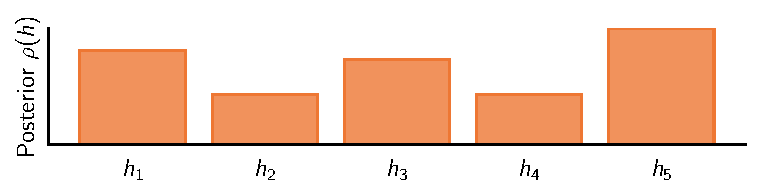
\includegraphics[width=0.8\linewidth]{figures/distribution_post.pdf}
  \end{figure}

\end{xframe}

%%%%%%%%%%%%%%%%%%%%%%%%%%%%%%%%%%%%%%%%%%%%%%%%%%%%%%%%%%%%%%%%%%%%%%%%%%%%%%%

\begin{xframe}{{\it PAC}-Bayesian Generalization Bound}

  \vfill

  \begin{figure}
  \includestandalone[width=0.9\linewidth]{figures/distribution.tex}
  \end{figure}
  
  \vfill

\end{xframe}

%%%%%%%%%%%%%%%%%%%%%%%%%%%%%%%%%%%%%%%%%%%%%%%%%%%%%%%%%%%%%%%%%%%%%%%%%%%%%%%

\begin{xframe}{{\it PAC}-{\bf Bayesian} Generalization Bound}

  \vspace{-0.3cm}

  \only<1->{
  \begin{xblock}{}
  {\bf A \red{Probably} \blue{Approximately} \green{Correct} (\red{P}\blue{A}\green{C}) generalization bound}~{\small\citep{Valiant1984}}

    {\small For any $\D$ on $\X\times\Y$, for all $\delta\in(0, 1]$, we have}\\[-0.6cm]
    \begin{align*}
      \red{\PP_{\dS\sim\D^\m}}\,\Big[\; \green{\Risk_{\D}(\black{\h_{\dS}})} \,\le\, \blue{\Risk_{\dS}(\black{\h_{\dS}}) + \Phi(\black{\h_{\dS}}, \dS, \delta)} \;\Big]\,\red{\ge 1-\delta}
    \end{align*}
    \scalebox{0.9}{With \red{high probability (at least $1{-}\delta$)}, the \green{\bf risk} of the classifier $h_\dS$ is less than \blue{$\Risk_{\dS}(\black{\h_{\dS}}) + \Phi(\black{\h_{\dS}}, \dS, \delta)$}}
  \end{xblock}
  }

  \only<2->{
  \begin{redbox}{}
    \textbf{\red{P}\blue{A}\green{C}-\orange{Bayesian} Bound}~{\scriptsize\citep{ShaweTaylorWilliamson1997,McAllester1998}}\\[-0.0cm]
    {\scriptsize For any $\D$ on $\X\times\Y$, for any hypothesis set $\H$, for any prior $\P$ on $\H$, for any $\delta\in(0, 1]$, we have}\\[-0.6cm]
    \begin{align*}
      \hspace{-0.3cm}\red{\PP_{\dS\sim\D^\m}}\Bigg[\, \forall \orange{\Q}\text{ on }\H,\ \underbrace{\EE_{h\sim \orange{\Q}}\green{\Risk_{\D}(\black{h})}}_{\mathclap{\text{\green{\bf Expected true risk}}}} \ \ \quad\le\quad  \underbrace{\EE_{h\sim \orange{\Q}}\blue{\Risk_{\dS}(\black{h})}}_{\mathclap{\text{\hspace{-0.4cm}\blue{\bf Expected empirical risk}}}} \quad+\quad \underbrace{\blue{\sqrt{\frac{1}{2m}\Big[\underbrace{\KL(\orange\Q\|\black{\P})}_{\mathclap{\text{\bf \ \ KL divergence}}} +\ln\frac{2\sqrt{m}}{\delta}\Big]}}}_{\mathclap{\text{\blue{\bf Complexity}}}} \,\Bigg]\red{\;\ge\; 1{-}\delta}
    \end{align*}
    
    \vspace{-0.2cm}
    {\small where $\KL(\Q\|\P)=\EE_{h\sim\Q}\ln\frac{\Q(h)}{\P(h)}$}
  \end{redbox}
  }
 
\end{xframe}

%%%%%%%%%%%%%%%%%%%%%%%%%%%%%%%%%%%%%%%%%%%%%%%%%%%%%%%%%%%%%%%%%%%%%%%%%%%%%%%
%%%%%%%%%%%%%%%%%%%%%%%%%%%%%%%%%%%%%%%%%%%%%%%%%%%%%%%%%%%%%%%%%%%%%%%%%%%%%%%
%%%%%%%%%%%%%%%%%%%%%%%%%%%%%%%%%%%%%%%%%%%%%%%%%%%%%%%%%%%%%%%%%%%%%%%%%%%%%%%
%%%%%%%%%%%%%%%%%%%%%%%%%%%%%%%%%%%%%%%%%%%%%%%%%%%%%%%%%%%%%%%%%%%%%%%%%%%%%%%

\section{Self-bounding Algorithms for the Majority Vote}
\begin{xtitle}

\vspace{3cm}

{\huge Self-bounding Algorithms\\ for the Majority Vote}\\
{\small Based on the Minimization of PAC-Bayesian Bounds}

\vspace{3cm}

\xscalebox{0.65}{
\begin{center}
\mbox{\hspace{-4.3cm}\small\citeauthor{ZantedeschiViallardMorvantEmonetHabrardGermainGuedj2021}}\\
\mbox{\hspace{-4cm}\citetitle{ZantedeschiViallardMorvantEmonetHabrardGermainGuedj2021}}\\
\mbox{\citedetails{ZantedeschiViallardMorvantEmonetHabrardGermainGuedj2021} (\citeyear{ZantedeschiViallardMorvantEmonetHabrardGermainGuedj2021})}
\end{center}
}
\end{xtitle}

%%%%%%%%%%%%%%%%%%%%%%%%%%%%%%%%%%%%%%%%%%%%%%%%%%%%%%%%%%%%%%%%%%%%%%%%%%%%%%%
%%%%%%%%%%%%%%%%%%%%%%%%%%%%%%%%%%%%%%%%%%%%%%%%%%%%%%%%%%%%%%%%%%%%%%%%%%%%%%%
%%%%%%%%%%%%%%%%%%%%%%%%%%%%%%%%%%%%%%%%%%%%%%%%%%%%%%%%%%%%%%%%%%%%%%%%%%%%%%%
%%%%%%%%%%%%%%%%%%%%%%%%%%%%%%%%%%%%%%%%%%%%%%%%%%%%%%%%%%%%%%%%%%%%%%%%%%%%%%%

\begin{xframe}{Majority Vote}
   
    \vspace{0.3cm}
       
    \textbf{Our Model: }Majority vote on $\H$
    
    \vspace{0.3cm}

    \xscalebox{1.3}{
        \includestandalone{figures/mv_}
    }

    \vspace{0.3cm}

    \begin{xblock}{}
      {\bf The voters}: Let $\H$ the set of voters, where $\black{\h_1(), \h_2(), \h_3()}$ are ``simple'' functions
    \end{xblock}
    
    \vspace{0.3cm}
    
    \xscalebox{1.3}{
    \hspace{0.2cm}
    \includestandalone{figures/mv}
    }

  \end{xframe}

%%%%%%%%%%%%%%%%%%%%%%%%%%%%%%%%%%%%%%%%%%%%%%%%%%%%%%%%%%%%%%%%%%%%%%%%%%%%%%%

\begin{xframe}{Majority Vote Learning}
    
    \vspace{0.3cm}
    
    \textbf{Our model: }Majority vote on $\H$
    
    \vspace{0.3cm}

    \xscalebox{1.3}{
        \includestandalone{figures/mv_}
    }

    \vspace{0.3cm}
    
    \begin{xblock}{}
      Combine the decision of the voters $\h: \X \to \{-1, +1\}$ with a posterior distribution $\Q$ on $\H$
    \end{xblock}
        
    \vspace{-0.2cm}
    
    \begin{align*}
        \forall \x\in\X,\quad \MVQ(\x) = \sign\LB \sum_{\h\in\H}\Q(\h)\h(\x)\RB
    \end{align*}

    \begin{redbox}{}
    {\bf\red{Objective:}} Find a posterior distribution $\Q$ minimizing the 

    \vspace{-0.6cm}
    \begin{align*}
    \text{\bf True Risk of the Majority Vote}\quad \Risk_{\D}(\MVQ) =\ \PP_{(\x, \y)\sim\D}\Big[   \MVQ(\x) \ne \y\Big]
    \end{align*}
    \end{redbox}
\end{xframe}

%%%%%%%%%%%%%%%%%%%%%%%%%%%%%%%%%%%%%%%%%%%%%%%%%%%%%%%%%%%%%%%%%%%%%%%%%%%%%%%

\begin{xframe}{Upper Bounds on the Majority Vote True Risk}

\vspace{-0.3cm}

\begin{xblock}{}
\red{\bf Drawback of the majority vote's true risk:} Difficult to minimize
\end{xblock}

\vspace{0.3cm}

{\bf  Joint error}\\[0.5cm]
\hspace{0.1cm}$\displaystyle  \green{e_{\D}(\Q)} = \PP_{(\x,\y)\sim\D, \h\sim\Q, \h'\sim\Q}\LB\h(\x) \ne \y, \h'(\x) \ne \y\RB$
    
\vspace{0.5cm}
    
{\bf Upper bound (surrogate) on the majority vote true risk}\\[0.5cm]
\hspace{0.1cm}$\displaystyle\green{\Risk_{\D}(\MVQ)} \le \green{4e_{\D}(\Q)}$

\vspace{0.5cm}

{\bf PAC-Bayesian bound on the majority vote true risk} {\scriptsize \citep{MasegosaLorenzenIgelSeldin2020}}

{\scriptsize For any distribution $\D$ on $\X{\times}\Y$, for any hypothesis set $\H$, for any prior distribution $\P$, for any $\delta \in (0, 1]$, with probability at least $1-\delta$ over the random choice of $\dS\sim\D^\m$, we have for all posterior $\Q$ on $\H$}\\[-0.5cm]
\begin{align*}
    \green{\Risk_{\D}(\MVQ)} \le \blue{4e_{\dS}(\Q)} + \blue{\sqrt{\frac{8}{m}\Big[\KL(\orange\Q\|\black{\P}) +\ln\frac{2\sqrt{m}}{\delta}\Big]}} \quad\text{\scriptsize with $\displaystyle\blue{e_{\dS}(\Q)} = \frac{1}{\m}\sum_{i=1}^{\m}\PP_{\h\sim\Q, \h'\sim\Q}\LB\h(\x_i) \ne \y_i, \h'(\x_i) \ne \y_i\RB$}
\end{align*}

\end{xframe}

%%%%%%%%%%%%%%%%%%%%%%%%%%%%%%%%%%%%%%%%%%%%%%%%%%%%%%%%%%%%%%%%%%%%%%%%%%%%%%%

\begin{xframe}{Surrogates on the Majority Vote True Risk}

\begin{enumerate}
    \item The surrogates are not precise for minimizing the empirical risk\\
    \begin{minipage}{0.50\linewidth}
        \begin{center}
        Minimizing {\it empirical} joint error
        \end{center}
        \begin{align*}
        \min_{\Q} \LC \blue{4e_{\dS}(\Q)} \RC
        \end{align*}
    \end{minipage}
    \hfill
    \begin{minipage}{0.49\linewidth}
    \begin{figure}
        \centering
        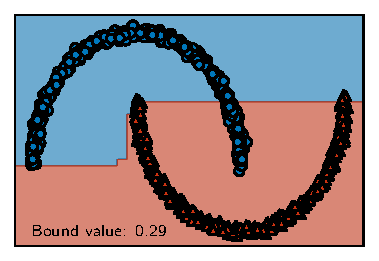
\includegraphics[width=0.7\linewidth]{figures/moons_risk.pdf}
    \end{figure}
    \end{minipage}

\item Even less precise when minimizing generalization bounds with a self-bounding algorithm\\
\begin{minipage}{0.50\linewidth}
\begin{center}
Self-bounding algorithm
\end{center}
\begin{align*}
\min_{\Q} \LC \blue{4e_{\dS}(\Q)} + \blue{\sqrt{\frac{8}{m}\Big[\KL(\orange\Q\|\black{\P}) +\ln\frac{2\sqrt{m}}{\delta}\Big]}} \RC
\end{align*}
\end{minipage}
\hfill
\begin{minipage}{0.49\linewidth}
\begin{figure}
    \centering
    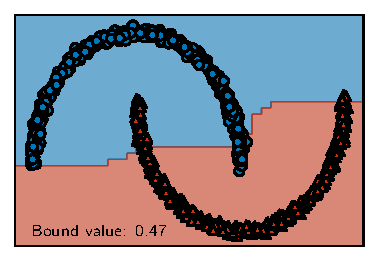
\includegraphics[width=0.7\linewidth]{figures/moons_bound.pdf}
\end{figure}
\end{minipage}
\end{enumerate}
\end{xframe}

%%%%%%%%%%%%%%%%%%%%%%%%%%%%%%%%%%%%%%%%%%%%%%%%%%%%%%%%%%%%%%%%%%%%%%%%%%%%%%%

\begin{xframe}{Contributions on the {\it Stochastic} Majority Vote}

\vfill

\red{\bf Drawbacks of the majority vote:}\\[0.5cm]
\begin{itemize}

    \item[\red{\bf --} ] PAC-Bayesian generalization bounds are not necessarily tight (because of the surrogates)\\[0.3cm]
    
    \item[\red{\bf --} ] Self-bounding algorithms do not take full advantage of the combination of voters
\end{itemize}

\vfill

\begin{redbox}{}
\red{\bf Our Contribution: }
\begin{enumerate}
    \item We introduce the stochastic majority vote {\scriptsize (randomness involved for each input)}\\[-0.3cm]
    \item We derive a PAC-Bayesian bound for the stochastic majority vote\\ {\scriptsize (with a closed-form solution for the empirical risk!)}\\[-0.3cm]
    \item We have a self-bounding algorithm (by minimizing the PAC-Bayesian bound)
\end{enumerate}    
\end{redbox}

\vfill

\end{xframe}

%%%%%%%%%%%%%%%%%%%%%%%%%%%%%%%%%%%%%%%%%%%%%%%%%%%%%%%%%%%%%%%%%%%%%%%%%%%%%%%

\begin{xframe}{Our Contribution -- {\small Stochastic Majority Vote}}

\vfill
\begin{figure}
    \centering
    \includestandalone[width=0.97\linewidth]{figures/sto_mv}
\end{figure}
\vfill

\end{xframe}

%%%%%%%%%%%%%%%%%%%%%%%%%%%%%%%%%%%%%%%%%%%%%%%%%%%%%%%%%%%%%%%%%%%%%%%%%%%%%%%

\begin{xframe}{Our Contribution -- {\small Stochastic Majority Vote}}

    \vspace{-0.2cm}

  \begin{figure}
   \centering
   \includestandalone[width=0.44\linewidth]{figures/sto_mv_weight}
  \end{figure}

  \vspace{-0.2cm}

  \begin{redbox}{}
  {\bf For stochastic majority vote:} Find a {\it hyper-posterior} $\hyperQ$ minimizing $\EE_{\Q\sim\hyperQ}\green{\Risk_{\D}(\black{\MVQ})}$
  \end{redbox}

\end{xframe}

%%%%%%%%%%%%%%%%%%%%%%%%%%%%%%%%%%%%%%%%%%%%%%%%%%%%%%%%%%%%%%%%%%%%%%%%%%%%%%%

\begin{xframe}{Our Contribution -- {\small Bound and Algorithm for the Stochastic Majority Vote}}

    \vfill

    \begin{redbox}{}
        \red{\bf PAC-Bayesian bound for the stochastic majority vote}
        
        {\scriptsize For any distribution $\D$ on $\X{\times}\Y$, for any finite hypothesis set $\H$, for any hyper-prior distribution $\hyperP$, for any $\delta \in (0, 1]$, with probability at least $1-\delta$ over the random choice of $\dS\sim\D^\m$, we have for all hyper-posteriors $\hyperQ$ on $\H$}\\[-0.5cm]
     \begin{align*}
       \EE_{\Q\sim\hyperQ}\green{\Risk_{\D}(\MVQ)} \le \EE_{\Q\sim\hyperQ}\blue{\Risk_{\dS}(\MVQ) + \sqrt{\tfrac{1}{2\m}\LB\KL(\hyperQ\|\hyperP) +\ln\tfrac{2\sqrt{\m}}{\delta}\RB}}
    \end{align*}
    \vspace{-0.2cm}
    
       \red{\bf Self-bounding algorithm}
       \vspace{-0.5cm}
       
       \begin{align*}
       \min_{\hyperQ}\Bigg\{ \EE_{\Q\sim\hyperQ}\blue{\Risk_{\dS}(\MVQ) + \sqrt{\tfrac{1}{2\m}\LB\KL(\hyperQ\|\hyperP) +\ln\tfrac{2\sqrt{\m}}{\delta}\RB}}\Bigg\}
        \end{align*}
    \end{redbox}
    
    \vspace{-0.1cm}
    \begin{xblock}{}
    \red{\bf Issue:} The right-hand side of the inequality is not computable (in general)\\[0.2cm]
    \red{$\Rightarrow$} Special case of hyper-priors $\hyperP$ and hyper-posteriors $\hyperQ$ with a computable bound
    \end{xblock}
    
    \vfill
    
\end{xframe}

%%%%%%%%%%%%%%%%%%%%%%%%%%%%%%%%%%%%%%%%%%%%%%%%%%%%%%%%%%%%%%%%%%%%%%%%%%%%%%%

\begin{xframe}{Our Contribution -- {\small Dirichlet Distribution}}

\begin{redbox}{}
\centering
Hyper-posterior $\hyperQ$ = Dirichlet distribution $\Dir(\paramDir)$
\end{redbox}

\vspace{-0.3cm}

\begin{center}
\xscalebox{0.65}{
\begin{figure}
\centering
\begin{subfigure}{0.32\textwidth}
    \only<1->{
    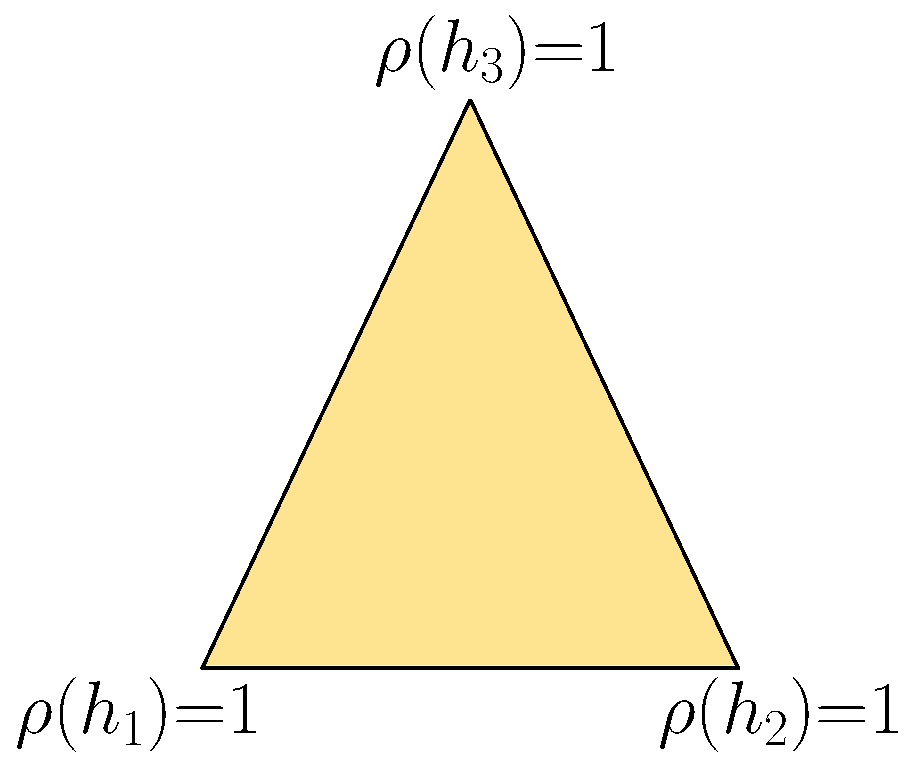
\includegraphics[width=\textwidth]{figures/dirichlet_1_1_1.pdf}
    \caption{$\paramDir=[1, 1, 1]^{\top}$}
    }
\end{subfigure}
\hfill
\begin{subfigure}{0.32\textwidth}
    \only<2->{
    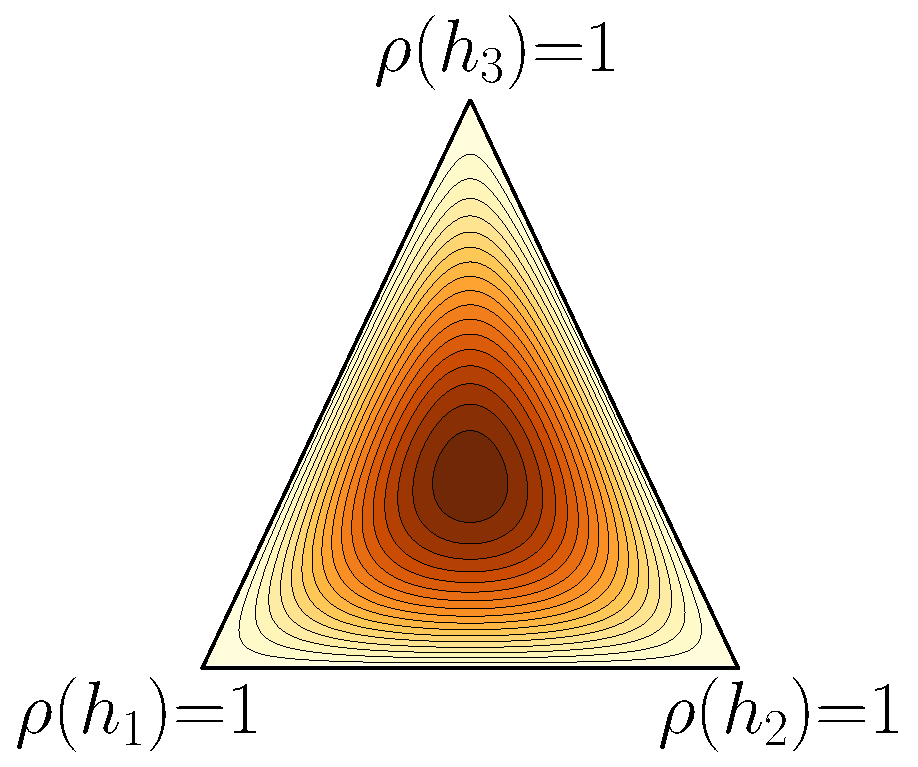
\includegraphics[width=\textwidth]{figures/dirichlet_2_2_2.pdf}
    \caption{$\paramDir=[2, 2, 2]^{\top}$}
    }
\end{subfigure}
\hfill
\begin{subfigure}{0.32\textwidth}
    \only<2->{
    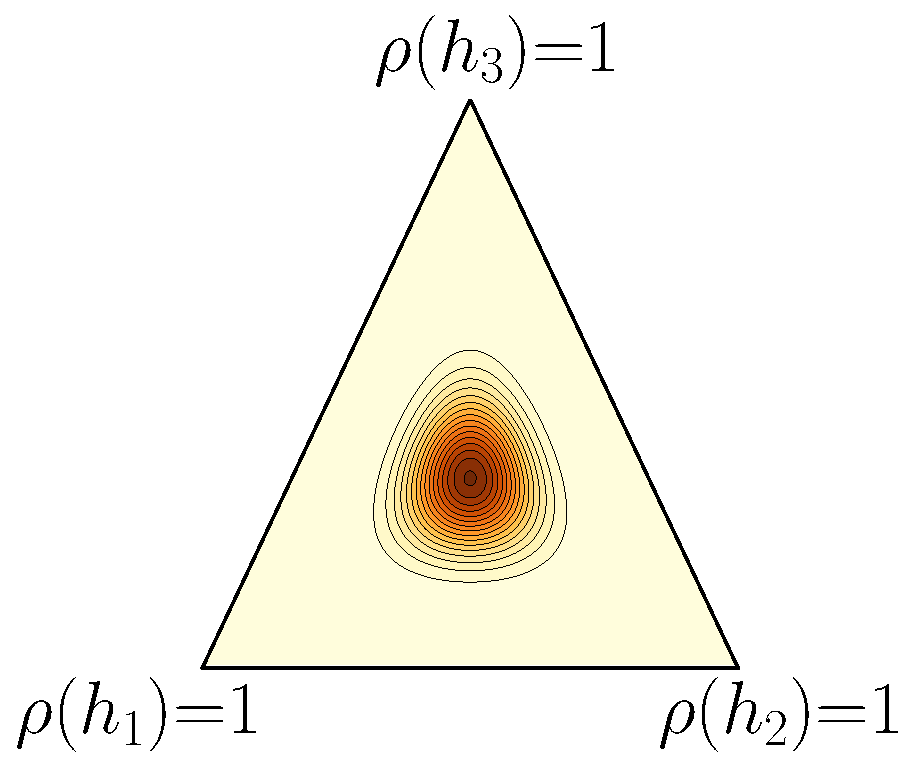
\includegraphics[width=\textwidth]{figures/dirichlet_10_10_10.pdf}
    \caption{$\paramDir=[10, 10, 10]^{\top}$}
    }
\end{subfigure}

\begin{subfigure}{0.32\textwidth}
    \only<3->{
    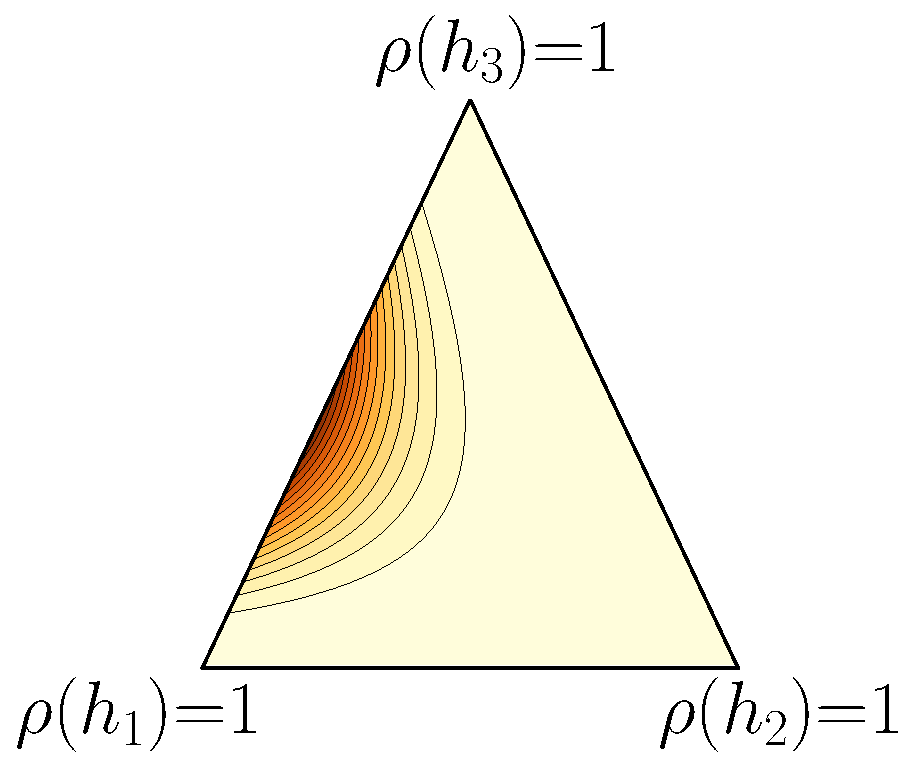
\includegraphics[width=\textwidth]{figures/dirichlet_5_1_4.pdf}
    \caption{$\paramDir=[5, 1, 4]^{\top}$}
    }
\end{subfigure}
\hfill
\begin{subfigure}{0.32\textwidth}
    \only<3->{
    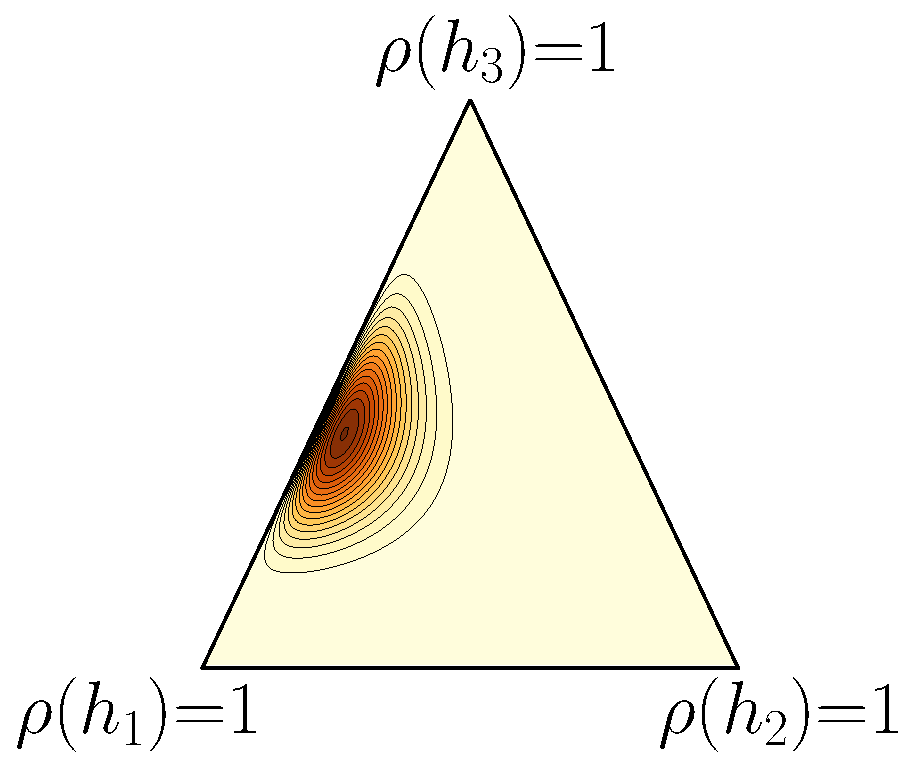
\includegraphics[width=\textwidth]{figures/dirichlet_10_2_8.pdf}
    \caption{$\paramDir=[10, 2, 8]^{\top}$}
    }
\end{subfigure}
\hfill
\begin{subfigure}{0.32\textwidth}
    \only<3->{
    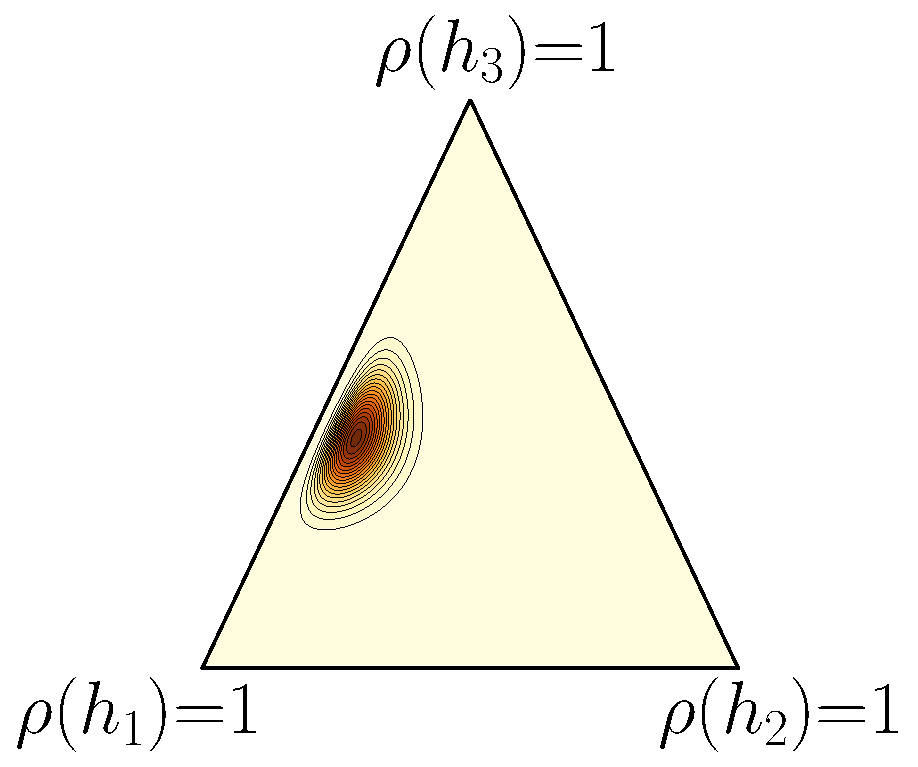
\includegraphics[width=\textwidth]{figures/dirichlet_25_5_20.pdf}
    \caption{$\paramDir=[25, 5, 20]^{\top}$}
    }
\end{subfigure}
\end{figure}
}
\end{center}

\end{xframe}

%%%%%%%%%%%%%%%%%%%%%%%%%%%%%%%%%%%%%%%%%%%%%%%%%%%%%%%%%%%%%%%%%%%%%%%%%%%%%%%

\begin{xframe}{Our Contribution -- {\small Computation of the Empirical Risk}}

\vfill

\begin{redbox}{}

\xscalebox{1.0}{For each example $(\x_i, \y_i)$, the parameters $\paramDir$ are separated into two subsets:}\\[0.2cm]
\xscalebox{1.0}{\begin{itemize}
    \item $\Tbb(\x_i,\y_i)$ = \xscalebox{0.88}{Indices of the Dirichlet parameters of the voters that \textbf{correctly classify} $(\x_i, \y_i)$}
    \item $\Fbb(\x_i,\y_i)$ = \xscalebox{0.88}{Indices of the Dirichlet parameters of the voters that {\bf misclassify} $(\x_i, \y_i)$}
\end{itemize}}

\end{redbox}

\vspace{0.2cm}

\begin{xblock}{}
\red{\bf Closed-form solution of the empirical risk {\scriptsize {\bf (in binary classification)}}}
\vspace{-0.2cm}
\begin{align*}
    \EE_{\Q\sim\hyperQ}\blue{\Risk_{\dS}(\MVQ)} = \frac{1}{\m}\sum_{i=1}^{\m} I_{0.5}\LP\ \sum_{\red{j} \in \Tbb(\x_i,\y_i)} \sparamDir_{\red{j}}, \sum_{\red{j} \in \Fbb(\x_i,\y_i)} \sparamDir_{\red{j}}\RP
\end{align*}

\vspace{-0.1cm}
\xscalebox{0.9}{with $I_{0.5}()$ the regularized incomplete beta function evaluated at $0.5$}
\end{xblock}

\vfill

\end{xframe}

%%%%%%%%%%%%%%%%%%%%%%%%%%%%%%%%%%%%%%%%%%%%%%%%%%%%%%%%%%%%%%%%%%%%%%%%%%%%%%%

\begin{xframe}{Advantages and Limitations of our Approach}

\vspace{-0.7cm}

\begin{center}
\xscalebox{1.0}{
\begin{figure}
\centering
\begin{subfigure}{0.32\textwidth}
    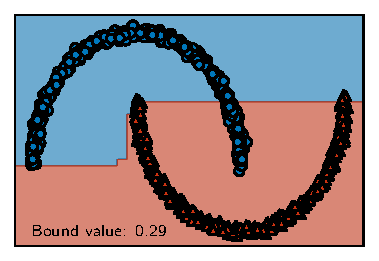
\includegraphics[width=\textwidth]{figures/moons_risk.pdf}
    \caption{{\bf Majority Vote}\\ Risk minimization}
\end{subfigure}
\hfill
\begin{subfigure}{0.32\textwidth}
    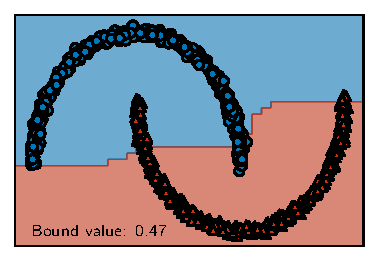
\includegraphics[width=\textwidth]{figures/moons_bound.pdf}
    \caption{{\bf Majority Vote}\\ Self-bounding algorithm}
\end{subfigure}
\hfill
\begin{subfigure}{0.32\textwidth}
    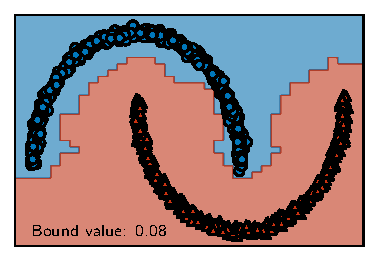
\includegraphics[width=\textwidth]{figures/moons_ours.pdf}
    \caption{{\bf Stochastic Majority Vote}\\ Self-bounding algorithm}
\end{subfigure}
\end{figure}
}
\end{center}

\vspace{-0.6cm}

\red{\textbf{Advantages: }}\\[0.1cm] 
\begin{xitemize}
    \item[\green{\bf +}] We obtain tight PAC-Bayesian generalization bounds
    \item[\green{\bf +}] We have a self-bounding algorithm
    \item[\green{\bf +}] Our contribution is extended to multi-class setting
\end{xitemize}

\vspace{0.2cm}

\red{\textbf{Limitations: }}\\[0.1cm]
\begin{xitemize}
    \item[\red{\bf --} ] The majority vote is stochastic
    \item[\red{$\Rightarrow$}] The PAC-Bayesian bound does not consider a unique majority vote
\end{xitemize}

\vfill

\end{xframe}

%%%%%%%%%%%%%%%%%%%%%%%%%%%%%%%%%%%%%%%%%%%%%%%%%%%%%%%%%%%%%%%%%%%%%%%%%%%%%%%
%%%%%%%%%%%%%%%%%%%%%%%%%%%%%%%%%%%%%%%%%%%%%%%%%%%%%%%%%%%%%%%%%%%%%%%%%%%%%%%
%%%%%%%%%%%%%%%%%%%%%%%%%%%%%%%%%%%%%%%%%%%%%%%%%%%%%%%%%%%%%%%%%%%%%%%%%%%%%%%
%%%%%%%%%%%%%%%%%%%%%%%%%%%%%%%%%%%%%%%%%%%%%%%%%%%%%%%%%%%%%%%%%%%%%%%%%%%%%%%

\section{A Practical Perspective for Disintegrated PAC-Bayesian Bounds}
\begin{xtitle}

\vspace{3cm}

{\huge A Practical Perspective for\\ Disintegrated PAC-Bayesian Bounds}\\

\vspace{3.5cm}

\xscalebox{0.7}{
\begin{center}
{\small\citeauthor{ViallardGermainHabrardMorvant2022}}\\
\mbox{\hspace{-1.8cm}\citetitle{ViallardGermainHabrardMorvant2022}}\\
\citedetails{ViallardGermainHabrardMorvant2022}
\end{center}
}
\end{xtitle}

%%%%%%%%%%%%%%%%%%%%%%%%%%%%%%%%%%%%%%%%%%%%%%%%%%%%%%%%%%%%%%%%%%%%%%%%%%%%%%%
%%%%%%%%%%%%%%%%%%%%%%%%%%%%%%%%%%%%%%%%%%%%%%%%%%%%%%%%%%%%%%%%%%%%%%%%%%%%%%%
%%%%%%%%%%%%%%%%%%%%%%%%%%%%%%%%%%%%%%%%%%%%%%%%%%%%%%%%%%%%%%%%%%%%%%%%%%%%%%%
%%%%%%%%%%%%%%%%%%%%%%%%%%%%%%%%%%%%%%%%%%%%%%%%%%%%%%%%%%%%%%%%%%%%%%%%%%%%%%%

\begin{xframe}{{\it Disintegrated} {\it PAC}-Bayesian Generalization Bound}

\only<1->{
\begin{block}{}
    \vspace{-0.2cm}
    {\scriptsize For any $\D$ on $\X\times\Y$, for any hypothesis set $\H$, for any prior $\P$ on $\H$, for any $\delta\in(0, 1]$, we have}\\[-0.6cm]
    \begin{align*}
      \red{\PP_{\dS\sim\D^\m}}\Bigg[\, \forall \orange{\Q}\text{ on }\H,\quad \EE_{h\sim \orange{\Q}}\green{\Risk_{\D}(\black{h})} \le \EE_{h\sim \orange{\Q}}\blue{\Risk_{\dS}(\black{h})} +  \blue{\sqrt{\frac{1}{2m}\Big[\KL(\orange\Q\|\black{\P}) +\ln\frac{2\sqrt{m}}{\delta}\Big]}} \,\Bigg]\red{\;\ge\; 1{-}\delta}
    \end{align*}
    
    \vspace{-0.3cm}
\end{block}
}

\vspace{0.3cm}

\only<2->{
\begin{redbox}{}
\textbf{{\it Disintegrated} \red{P}\blue{A}\green{C}-\orange{Bayesian} Bound} {\scriptsize\citep{Catoni2007,BlanchardFleuret2007,RivasplataKuzborskijSzepesvariShaweTaylor2020}}\\[-0.2cm]

{\scriptsize For any $\D$ on $\X\times\Y$, for any hypothesis set $\H$, for any prior $\P$ on $\H$, for any $\delta\in(0, 1]$, for any algorithm $A$, we have}\\[-0.6cm]
\begin{align*}
\red{\PP_{\dS\sim\D^\m,\ \black{\h}\sim\AQ}}\Bigg[\phantom{\, \forall \orange{\Q}\text{ on }\H, \EE_{h\sim \orange{\Q}}}\green{\Risk_{\D}(\black{h})} \le \phantom{\EE_{h\sim \orange{\Q}}}\blue{\Risk_{\dS}(\black{h})} +  \blue{\sqrt{\frac{1}{2m}\Big[ \ln\frac{\AQ(\black{\h})}{\P(\black{\h})} +\ln\frac{2\sqrt{m}}{\delta}\Big]_{+}}} \,\Bigg]\red{\;\ge\; 1{-}\delta}
\end{align*}
{\small where $\AQ \defeq A(\dS, \P)$ is output by the deterministic algorithm $A$ and $[a]_+ = \max(0,a)$}
\end{redbox}
}
\end{xframe}

%%%%%%%%%%%%%%%%%%%%%%%%%%%%%%%%%%%%%%%%%%%%%%%%%%%%%%%%%%%%%%%%%%%%%%%%%%%%%%%

\begin{xframe}{A Practical Perspective for Disintegrated PAC-Bayesian Bounds}

\begin{xblock}{}
\textbf{{\it Disintegrated} \red{P}\blue{A}\green{C}-\orange{Bayesian} Bound} {\scriptsize\citep[Example based on][]{RivasplataKuzborskijSzepesvariShaweTaylor2020}}\\

{\scriptsize For any $\D$ on $\X\times\Y$, for any hypothesis set $\H$, for any prior $\P$ on $\H$, for any $\delta\in(0, 1]$, for any algorithm $A$, we have}\\[-0.6cm]
\begin{align*}
\red{\PP_{\dS\sim\D^\m,\ \black{\h}\sim\AQ}}\Bigg[\, \green{\Risk_{\D}(\black{h})} \le \blue{\Risk_{\dS}(\black{h})} +  \blue{\sqrt{\frac{1}{2m}\Big[ \ln\frac{\AQ(\black{\h})}{\P(\black{\h})} +\ln\frac{2\sqrt{m}}{\delta}\Big]_{+}}} \,\Bigg]\red{\;\ge\; 1{-}\delta}
\end{align*}
{\small where $\AQ \defeq A(\dS, \P)$ is output by the deterministic algorithm $A$ and $[a]_+ = \max(0,a)$}
\end{xblock}

\vspace{-0.2cm}

\begin{redbox}{}
\vspace{-0.1cm}
\red{\bf A practical perspective {\footnotesize (derandomization of the PAC-Bayesian bounds)}}
\begin{enumerate}
    \item Sampling a learning sample $\dS$ from $\D$
    \item Sampling a hypothesis $\h$ from $\AQ$
    \item \red{With high probability (at least $1-\delta$),} a bound holds, \eg, we have\\[-0.6cm]
    \begin{align*}
    \green{\Risk_{\D}(\black{h})} \le \blue{\Risk_{\dS}(\black{h})} +  \blue{\sqrt{\frac{1}{2m}\Big[ \ln\frac{\AQ(\black{\h})}{\P(\black{\h})} +\ln\frac{2\sqrt{m}}{\delta}\Big]_{+}}}
    \end{align*}
    \vspace{-0.6cm}
\end{enumerate}
\end{redbox}
\end{xframe}

%%%%%%%%%%%%%%%%%%%%%%%%%%%%%%%%%%%%%%%%%%%%%%%%%%%%%%%%%%%%%%%%%%%%%%%%%%%%%%%

\begin{xframe}{Advantages and Drawbacks of the Disintegrated PAC-Bayesian Bounds}

\begin{xblock}{}
\textbf{{\it Disintegrated} \red{P}\blue{A}\green{C}-\orange{Bayesian} Bound} {\scriptsize\citep[Example based on][]{RivasplataKuzborskijSzepesvariShaweTaylor2020}}\\

{\scriptsize For any $\D$ on $\X\times\Y$, for any hypothesis set $\H$, for any prior $\P$ on $\H$, for any $\delta\in(0, 1]$, for any algorithm $A$, we have}\\[-0.6cm]
\begin{align*}
\red{\PP_{\dS\sim\D^\m,\ \black{\h}\sim\AQ}}\Bigg[\, \green{\Risk_{\D}(\black{h})} \le \blue{\Risk_{\dS}(\black{h})} +  \blue{\sqrt{\frac{1}{2m}\Big[ \ln\frac{\AQ(\black{\h})}{\P(\black{\h})} +\ln\frac{2\sqrt{m}}{\delta}\Big]_{+}}} \,\Bigg]\red{\;\ge\; 1{-}\delta}
\end{align*}
{\small where $\AQ \defeq A(\dS, \P)$ is output by the deterministic algorithm $A$ and $[a]_+ = \max(0,a)$}
\end{xblock}

\vspace{-0.2cm}

\begin{redbox}{}
\begin{enumerate}
    \item \red{\bf Advantage:} Bound for a {\it unique} hypothesis $\h\sim\AQ$
    \item These bounds have not been studied in practice
    \item \red{\bf Drawback:} The term depends $\blue{\ln\frac{\AQ(\black{\h})}{\P(\black{\h})}}$ on the hypothesis $\h\sim\AQ$ 
    \item[\red{$\Rightarrow$}] Difficult to minimize (through a self-bounding algorithm)
\end{enumerate}
\end{redbox}
\end{xframe}

%%%%%%%%%%%%%%%%%%%%%%%%%%%%%%%%%%%%%%%%%%%%%%%%%%%%%%%%%%%%%%%%%%%%%%%%%%%%%%%

\begin{xframe}{Our Contribution -- {\small Practical Disintegrated PAC-Bayesian Bound}}

\vspace{-0.4cm}
\begin{xblock}{}
\xscalebox{0.95}{
\mbox{{\bf Our contribution: } Deriving disintegrated generalization bounds that are more easily minimizable}}
\end{xblock}

\begin{redbox}{}
\red{\bf New practical disintegrated bound}\\
{\scriptsize For any $\D$ on $\X\times\Y$, for any hypothesis set $\H$, for any prior $\P$ on $\H$, for any $\lambda\!>\!1$ for any $\delta\in(0, 1]$, for any algorithm $A$, we have}\\[-0.6cm]
\begin{align*}
    \red{\PP_{\dS\sim\D^{\m},\h\sim \AQ}}\LB\, \green{\Risk_{\D}(\h)} \le \blue{\Risk_{\dS}(\h)} + \blue{\sqrt{\frac{1}{2\m}\LB \Renyi_{\lambda}(\AQ\|\P)+ {\frac{2\lambda{-}1}{\lambda{-}1}}\ln\frac{2}{\delta}
 + \ln(2\sqrt{\m})\RB}} \RB \red{\ge\! 1{-}\delta}
\end{align*}
{\scriptsize where $\Renyi_{\lambda}(\AQ\|\P) \defeq \frac{1}{\lambda{-}1}\ln\!\LB \text{\small${\displaystyle \EE_{\h{\sim}\P}}$}\!\LB\!\frac{ \AQ(\h)}{\P(\h)}\RB^{\!\lambda}\RB$ and $\AQ \defeq A(\dS, \P)$ is output by the deterministic algorithm $A$}
\end{redbox}

\vspace{-0.2cm}

\begin{xblock}{}
{\bf The main difference: } Bound depends on the Rényi divergence $\Renyi_{\lambda}(\AQ\|\P)$ instead of $\ln\frac{\AQ(\h)}{\P(\h)}$

\vspace{-0.3cm}
\xscalebox{0.9}{
\begin{align*}
\red{\PP_{\dS\sim\D^\m,\ \black{\h}\sim\AQ}}\Bigg[\, \green{\Risk_{\D}(\black{h})} \le \blue{\Risk_{\dS}(\black{h})} +  \blue{\sqrt{\frac{1}{2m}\Big[ \ln\frac{\AQ(\black{\h})}{\P(\black{\h})} +\ln\frac{2\sqrt{m}}{\delta}\Big]_{+}}} \,\Bigg]\red{\;\ge\; 1{-}\delta}
\end{align*}
}

\vspace{-0.3cm}
\end{xblock}

\end{xframe}

%%%%%%%%%%%%%%%%%%%%%%%%%%%%%%%%%%%%%%%%%%%%%%%%%%%%%%%%%%%%%%%%%%%%%%%%%%%%%%%

\begin{xframe}{Our Contribution -- {\small Disintegrated PAC-Bayesian Bound Minimization Algorithm}}

\vspace{-0.1cm}

\only<1->{
{\bf Neural network learning algorithm with disintegrated PAC-Bayesian guarantees: }}

\begin{enumerate}
    \only<1->{
    \item Prior/posterior Gaussian distributions associated with the weights of the neural network

    \begin{figure}
    \includestandalone[width=0.9\linewidth]{figures/nn_sampling_1}
    \end{figure}}

    \only<2->{
    \item Learn $T$ priors $\Pbb=\{\P_\t\}_{\t=1}^{\iter}$ in $\iter$ epochs with $\dS'$\\[0.2cm]
    
    \includestandalone[width=0.5\linewidth]{figures/nn_sampling_2}
    }

    \only<3->{
    \item Learn the distribution $\AQ$ with $\dS$ from a prior $\P_\t$ selected with $\dS$
    \item Sample the neural network $\h \sim \AQ$

    \begin{figure}
    \includestandalone[width=0.9\linewidth]{figures/nn_sampling_3}
    \end{figure}
    }

\end{enumerate}

\vfill

\end{xframe}

%%%%%%%%%%%%%%%%%%%%%%%%%%%%%%%%%%%%%%%%%%%%%%%%%%%%%%%%%%%%%%%%%%%%%%%%%%%%%%%

\begin{xframe}{Our Contribution -- {\small Comparison with the Disintegrated PAC-Bayesian Bounds}}

\vspace{-0.3cm}

\begin{center}
{\bf Comparison with the disintegrated PAC-Bayesian bounds}
\end{center}

\vspace{-0.2cm}

\begin{minipage}{0.8\linewidth}
\begin{figure}[H]
    \centering
    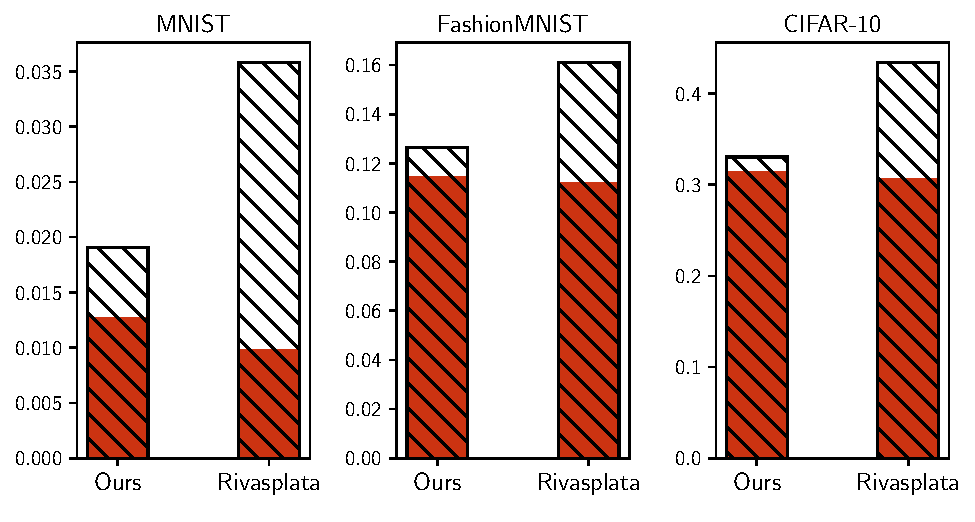
\includegraphics[width=0.9\linewidth]{figures/comparison_dis_bound_slides.pdf}
\end{figure}
\end{minipage}
\hfill
\begin{minipage}{0.19\linewidth}
\begin{figure}
\hspace{-0.6cm}\includestandalone[width=1.2\linewidth]{figures/comparison_legend}
\end{figure}
\end{minipage}

{\bf Conclusion:}
\begin{xitemize}
\item[\red{\bf --}] Test risk not always tighter\dots
\item[\green{\bf +}] Our bound is tighter in practice!
\end{xitemize}

\vfill

\end{xframe}

%%%%%%%%%%%%%%%%%%%%%%%%%%%%%%%%%%%%%%%%%%%%%%%%%%%%%%%%%%%%%%%%%%%%%%%%%%%%%%%

\begin{xframe}{The take-home Message}

\vfill

\red{\bf To sum up:}\\
\begin{xitemize}
    \item We are the first to optimize disintegrated PAC-Bayesian bounds\\[0.3cm]
    
    \item Our bound is tighter in practice compared to 
    \begin{enumerate}
        \item[(i)] the other disintegrated bound
        \item[(ii)] the classical PAC-Bayesian bound when sampling the networks
    \end{enumerate}
\end{xitemize}

\vspace{0.3cm}

\red{\bf Perspectives:} Disintegrated PAC-Bayesian bound for the stochastic majority vote!

\begin{redbox}{}
\red{\bf Disintegrated PAC-Bayesian bound for the stochastic majority vote}

{\scriptsize For any distribution $\D$ on $\X{\times}\Y$, for any finite set of voters $\H$, for any hyper-prior distribution $\hyperP$ on $\H$, for any $\lambda>1$, for any $\delta \in (0, 1]$, for any algorithm $A$, we have}\\[-0.6cm]
\begin{align*}
    &\red{\PP_{\dS\sim\D^{\m},\Q\sim \hyperAQ}}\Bigg[ 
    \green{\Risk_{\D}(\MVQ)} \le \blue{\Risk_{\dS}(\MVQ)} + \blue{\sqrt{\frac{1}{2\m}\Bigg[ \Renyi_{\lambda}(\hyperAQ\|\hyperP) + {\frac{2\lambda{-}1}{\lambda{-}1}}\ln\frac{2}{\delta} + \ln(2\sqrt{m})\Bigg]}} \Bigg] \red{\ge\! 1{-}\delta}
\end{align*}

\vspace{-0.3cm}
{\scriptsize where $\hyperAQ \defeq A(\dS, \hyperP)$ is output by the deterministic algorithm $A$}
\end{redbox}


\end{xframe}

%%%%%%%%%%%%%%%%%%%%%%%%%%%%%%%%%%%%%%%%%%%%%%%%%%%%%%%%%%%%%%%%%%%%%%%%%%%%%%%

\begin{xframe}{Drawbacks of the Current Generalization Bounds}

\vfill

{\bf Drawback:} The complexity is imposed by the generalization bounds
\begin{align*}
    \red{\PP_{\dS\sim\D^{\m},\h\sim \AQ}}\LB\, \green{\Risk_{\D}(\h)} \le \blue{\Risk_{\dS}(\h)} + \blue{\sqrt{\frac{1}{2\m}\LB \Renyi_{\lambda}(\AQ\|\P)+ {\frac{2\lambda{-}1}{\lambda{-}1}}\ln\frac{2}{\delta} + \ln(2\sqrt{\m})\RB}} \RB \red{\ge\! 1{-}\delta}
\end{align*}

\vspace{0.7cm}

{\bf To overcome this drawback:}\\[0.3cm]
\begin{xitemize}
    \item Some complexity measures have been empirically investigated\\ 
    \citep{JiangNeyshaburMobahiKrishnanBengio2020, DziugaiteDrouinNealRajkumarCaballeroWangMitliagkasRoy2020, JiangNatekarSharma2021}
    \item But these complexity measures are not involved in generalization bounds
    \item Prove generalization bounds with these complexity measures
\end{xitemize}

\vfill

\end{xframe}

%%%%%%%%%%%%%%%%%%%%%%%%%%%%%%%%%%%%%%%%%%%%%%%%%%%%%%%%%%%%%%%%%%%%%%%%%%%%%%%
%%%%%%%%%%%%%%%%%%%%%%%%%%%%%%%%%%%%%%%%%%%%%%%%%%%%%%%%%%%%%%%%%%%%%%%%%%%%%%%
%%%%%%%%%%%%%%%%%%%%%%%%%%%%%%%%%%%%%%%%%%%%%%%%%%%%%%%%%%%%%%%%%%%%%%%%%%%%%%%
%%%%%%%%%%%%%%%%%%%%%%%%%%%%%%%%%%%%%%%%%%%%%%%%%%%%%%%%%%%%%%%%%%%%%%%%%%%%%%%

\section{New Perspectives on Generalization}
\begin{xtitle}

\vspace{3cm}

{\huge New Perspectives on Generalization}\\
{\normalsize Thanks to the Disintegrated PAC-Bayesian Bounds}

\vspace{3cm}

\xscalebox{0.7}{
\begin{center}
\mbox{\hspace{-1.9cm}\small\citeauthor{ViallardEmonetHabrardMorvantZantedeschi2022}}\\
\mbox{\hspace{-1.3cm}\citetitle{ViallardEmonetHabrardMorvantZantedeschi2022}}\\
\citedetails{ViallardEmonetHabrardMorvantZantedeschi2022}
\end{center}
}
\end{xtitle}

%%%%%%%%%%%%%%%%%%%%%%%%%%%%%%%%%%%%%%%%%%%%%%%%%%%%%%%%%%%%%%%%%%%%%%%%%%%%%%%
%%%%%%%%%%%%%%%%%%%%%%%%%%%%%%%%%%%%%%%%%%%%%%%%%%%%%%%%%%%%%%%%%%%%%%%%%%%%%%%
%%%%%%%%%%%%%%%%%%%%%%%%%%%%%%%%%%%%%%%%%%%%%%%%%%%%%%%%%%%%%%%%%%%%%%%%%%%%%%%
%%%%%%%%%%%%%%%%%%%%%%%%%%%%%%%%%%%%%%%%%%%%%%%%%%%%%%%%%%%%%%%%%%%%%%%%%%%%%%%

\begin{xframe}{Teaser of the Contribution}

\vfill

\begin{redbox}{}
\red{\bf Our Contribution: {\small Generalization bounds with arbitrary complexity measures}}\\
\begin{enumerate}
    \item We consider the disintegrated PAC-Bayesian bounds
    \item \mbox{Let $\comp\!:\! \H{\times}(\X{\times}\Y)^\m {\to} \R$ a function}
    \item We are able to prove a generalization bound of the form
    \begin{align*}
        \red{\PP_{\dS\sim\Dcal^\m, \h\sim\AQ}}\Big[ \green{\Risk_{\D}(\h)} \le \blue{\Risk_{\dS}(\h) + }\underbrace{\blue{\PhiComp(\h,\dS,\delta)}}_{\hspace{0.3cm}\mathclap{\text{\bf Complexity Measure of }h}} \Big] \red{\ge 1{-}\delta}
    \end{align*}
\end{enumerate}    
\end{redbox}
\end{xframe}

%%%%%%%%%%%%%%%%%%%%%%%%%%%%%%%%%%%%%%%%%%%%%%%%%%%%%%%%%%%%%%%%%%%%%%%%%%%%%%%

\begin{xframe}{Contribution -- {\small Arbitrary Complexity Measures}}

\vfill

\begin{redbox}{}

\begin{xitemize}

\item The function $\comp\!:\! \H{\times}(\X{\times}\Y)^\m {\to} \R$ acts as a regularization term\\[-0.3cm]
    
    {\bf Examples of functions $\comp$:}
    \begin{align*}
         \comp(h_\wbf, \dS) {=} \|\wbf\|_{2}^2 \quad\quad\text{or}\quad\quad  \comp(h_\wbf, \dS) = \alpha\Risk_{\dSp}(h_\wbf) \quad\quad\text{or}\quad\quad \comp(h_\wbf, \dS) {=} 0
\end{align*}

\vspace{0.5cm}

\item Given $\comp$, let $\AQ$ be a Gibbs distribution defined as 
\begin{align*}
   \AQ(\black{h}) \propto \exp\LB-\alpha\Risk_{\dS}(h)-\comp(h, \dS)\RB
\end{align*}
where $\alpha\in\mathbb{R}_+$ is a concentration parameter

\end{xitemize}
\end{redbox}

\vfill

\end{xframe}

%%%%%%%%%%%%%%%%%%%%%%%%%%%%%%%%%%%%%%%%%%%%%%%%%%%%%%%%%%%%%%%%%%%%%%%%%%%%%%%

\begin{xframe}{Contribution -- {\small Arbitrary Complexity Measures}}

\vspace{-0.3cm}
\only<1>{
\begin{figure}[H]
    \includestandalone[scale=1.2]{figures/gibbs_1}
\end{figure}
}
\only<2>{
\begin{figure}[H]
    \includestandalone[scale=1.2]{figures/gibbs_2}
\end{figure}
}
\end{xframe}

%%%%%%%%%%%%%%%%%%%%%%%%%%%%%%%%%%%%%%%%%%%%%%%%%%%%%%%%%%%%%%%%%%%%%%%%%%%%%%%

\begin{xframe}{Contribution -- {\small Arbitrary Complexity Measures}}

\vfill

\begin{redbox}{}
\red{\bf Generalization bound with arbitrary complexity measures}\\
{\scriptsize For any distribution $\D$ on $\X\times\Y$, for any bounded hypothesis set $\H$, given the uniform prior distribution $\P$ on $\H$,  for any $\comp: \H{\times}(\X{\times}\Y)^\m{\to}\Rbb$, for any $\delta\in(0, 1]$, we have}
\begin{align*}
    \hspace{-0.3cm}\red{\PP_{\substack{\dS{\sim}\Dcal^\m\\ \h\black{'}{\sim}\P\\ \h{\sim}\AQ}}}\!\!
    \LB \green{\Risk_{\D}(\h)}{\le}\blue{\Risk_{\dS}(\h)}{+}\!\blue{\sqrt{\frac{1}{2\m}\LB \underbrace{\Big[\alpha\Risk_{\dS}(\black{\h{'}})+\comp(\black{\h'}\!,\dS)\Big]}_{\mathclap{\text{\bf Prior}}}{-}\underbrace{\Big[\alpha\Risk_{\dS}(\h)+\comp(\h,\dS)\Big]}_{\mathclap{\text{\bf Posterior}}}{+}\frac{8\sqrt{\m}}{\delta^2} \RB_{\!+}}} \RB\! \red{\ge\! 1{-}\delta}
\end{align*}
{\scriptsize where $[a]_+ = \max(0,a)$}
\end{redbox}

\vfill

\end{xframe}

%%%%%%%%%%%%%%%%%%%%%%%%%%%%%%%%%%%%%%%%%%%%%%%%%%%%%%%%%%%%%%%%%%%%%%%%%%%%%%%

\begin{xframe}{Contribution -- {\small Experiments on the Bounds' Tightness}}

\vspace{-0.3cm}

\begin{center}
{\bf Experiments on the bounds' tightness}
\end{center}

\vspace{-0.2cm}

\begin{minipage}{0.8\linewidth}
\begin{figure}[H]
    \centering
    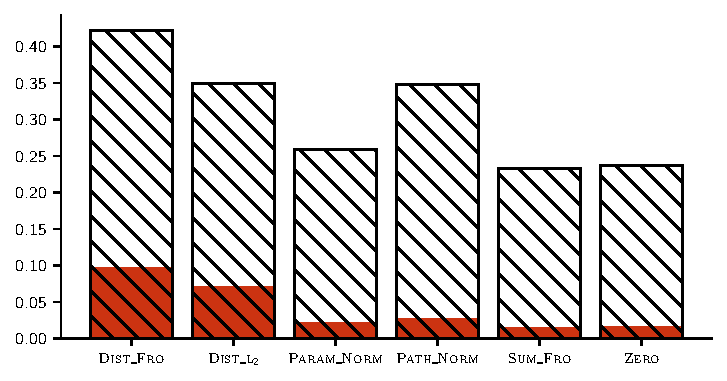
\includegraphics[width=0.9\linewidth]{figures/gap_mnist_min.pdf}
\end{figure}
\end{minipage}
\hfill
\begin{minipage}{0.19\linewidth}
\begin{figure}
\hspace{-0.6cm}\includestandalone[width=1.2\linewidth]{figures/gap_legend}
\end{figure}
\end{minipage}

\vspace{0.3cm}

{\bf Conclusion:}
\begin{xitemize}
\item The tightness depends on the chosen function $\comp$
\end{xitemize}

\end{xframe}

%%%%%%%%%%%%%%%%%%%%%%%%%%%%%%%%%%%%%%%%%%%%%%%%%%%%%%%%%%%%%%%%%%%%%%%%%%%%%%%

\begin{xframe}{Take-home Message}

\vspace{1cm}

\red{\bf To sum up: }
\begin{xitemize}
    \item We derive generalization bounds with arbitrary complexity measures
    \item We can retrieve the upper bounds of classical bounds\\
    (\eg, based on the Rademacher complexity)
\end{xitemize}

\vspace{1cm}

\red{\bf Perspectives: } 
\begin{xitemize}
    \item Design new complexity measures
    \item Extend the bound for other settings (\eg, non-iid setting)
\end{xitemize}

\end{xframe}

%%%%%%%%%%%%%%%%%%%%%%%%%%%%%%%%%%%%%%%%%%%%%%%%%%%%%%%%%%%%%%%%%%%%%%%%%%%%%%%

\section{PAC-Bayesian Bound for the Adversarial Robustness Setting}
\begin{xtitle}

\vspace{3.5cm}

{\huge PAC-Bayesian Bound for the Adversarial Robustness Setting}\\
{\normalsize (and its Derandomization)}

\vspace{2.5cm}

\xscalebox{0.7}{
\begin{center}
\mbox{\hspace{-1.9cm}\small\citeauthor{ViallardVidotHabrardMorvant2021}}\\
\mbox{\hspace{-1.3cm}\citetitle{ViallardVidotHabrardMorvant2021}}\\
\citedetails{ViallardVidotHabrardMorvant2021} (\citeyear{ViallardVidotHabrardMorvant2021})
\end{center}
}
\end{xtitle}

%%%%%%%%%%%%%%%%%%%%%%%%%%%%%%%%%%%%%%%%%%%%%%%%%%%%%%%%%%%%%%%%%%%%%%%%%%%%%%%

\begin{xframe}{Spotlight -- {\small PAC-Bayesian Bound for the Adversarial Robustness Setting}}

\vspace{-0.1cm}

\red{\bf 1} Self-bounding algorithm to robustify a model\\[-0.1cm]
\begin{figure}[H]
    \xscalebox{1.0}{
    \begin{center}
    \includestandalone[width=0.7\linewidth]{figures/robust}
    \end{center}
  }
\end{figure}

\vspace{-0.2cm}

\red{\bf 2} New adversarial risk for the majority vote

\vspace{-0.6cm}

\begin{align*}
    \green{\Risk_{\Dpert}(\MVQ)} \ =\  \PP_{((\x,\y), \epsilon)\sim \Dpert}\LB\MVQ(\x+\epsilon) \neq \y\RB\quad\text{and}\quad \blue{\Risk_{\dSpert}(\MVQ)} = \frac{1}{mn} \sum_{i=1}^\m\sum_{j=1}^n \indic\LB\MVQ(\x_i+\epsilon^i_j) \neq \y_i\RB
\end{align*}

\red{\bf 3} PAC-Bayesian generalization bound

\vspace{-0.6cm}
\begin{align*}
    \green{\Risk_{\Dpert}(\MVQ)} \le \blue{\Risk_{\dSpert}(\MVQ)} + \blue{\sqrt{\frac{2}{m}\LB \KL(\Q\|\P) + \ln\frac{m{+}1}{\delta}\RB}}
\end{align*}
\end{xframe}

%%%%%%%%%%%%%%%%%%%%%%%%%%%%%%%%%%%%%%%%%%%%%%%%%%%%%%%%%%%%%%%%%%%%%%%%%%%%%%%

\begin{xframe}{Perspectives -- {\small Disintegrated PAC-Bayesian bound for the adversarial robustness}}

\vspace{-0.3cm}

\begin{xblock}{}
\red{\bf Perspectives:} Disintegrated PAC-Bayesian bound for the adversarial robustness\\[0.5cm]

{\bf Adversarial true risk:} $\displaystyle\green{\RiskA_{\D}(\h)} = \PP_{(\x,\y)\sim\D}\LB\exists\epsilon\in\Xpert, \h(\x{+}\epsilon)\ne \y\RB$ {\scriptsize ($\Xpert$ the set of perturbations)}

{\bf Adversarial empirical risk:} $\displaystyle\blue{\RiskA_{\dS}(\h)} = \frac{1}{\m}\sum_{i=1}^{\m}\indic\LB\exists\epsilon\in\Xpert, \h(\x_i{+}\epsilon)\ne \y_i\RB$


\end{xblock}

\vspace{0.1cm}

\begin{redbox}{}
\red{\bf Disintegrated PAC-Bayesian bound for the adversarial robustness setting}

{\scriptsize For any distribution $\D$ on $\X{\times}\Y$, for any finite set of voters $\H$, for any prior distribution $\P$ on $\H$, for any $\lambda>1$, for any $\delta \in (0, 1]$, for any algorithm $A$, we have}\\[-0.6cm]
\begin{align*}
    &\red{\PP_{\dS\sim\D^{\m},\h\sim \AQ}}\Bigg[ 
    \green{\RiskA_{\D}(\h)} \le \blue{\RiskA_{\dS}(\h)} + \blue{\sqrt{\frac{1}{2\m}\Bigg[ \Renyi_{\lambda}(\AQ\|\P) + {\frac{2\lambda{-}1}{\lambda{-}1}}\ln\frac{2}{\delta} + \ln(2\sqrt{m})\Bigg]}} \Bigg] \red{\ge\! 1{-}\delta}
\end{align*}
\end{redbox}

\vfill

\end{xframe}

%%%%%%%%%%%%%%%%%%%%%%%%%%%%%%%%%%%%%%%%%%%%%%%%%%%%%%%%%%%%%%%%%%%%%%%%%%%%%%%

\section{Conclusion and Perspectives}
\begin{xtitle}
{\huge Conclusion and Perspectives}
\end{xtitle}

%%%%%%%%%%%%%%%%%%%%%%%%%%%%%%%%%%%%%%%%%%%%%%%%%%%%%%%%%%%%%%%%%%%%%%%%%%%%%%%

\begin{xframe}{Conclusion -- {\small Summary of the Contributions}}

\vspace{0.3cm}

{\bf What I presented:}\\[0.5cm]
\begin{enumerate}
\item PAC-Bayesian bound and a self-bounding algorithm for the {\it stochastic} majority vote \red{\footnotesize\citep[NeurIPS 2021,][]{ZantedeschiViallardMorvantEmonetHabrardGermainGuedj2021}}\\[0.3cm]  
\item New disintegrated PAC-Bayesian bounds that are the tightest in practice \red{\footnotesize (Submitted)}\\[0.3cm]

\item Generalization bound with a user-defined complexity measure \red{\footnotesize (Submitted)}\\[0.3cm]
\item First PAC-Bayesian bound for the adversarial robustness setting\\
\red{\footnotesize\citep[NeurIPS 2021,][]{ViallardVidotHabrardMorvant2021}}
\end{enumerate}

\vspace{0.5cm}

{\bf What I did not present:}\\[0.5cm]
\begin{enumerate}
\setcounter{enumi}{4}
\item Self-bounding algorithms for the (non-stochastic) majority vote\\\red{\footnotesize\citep[ECML 2021,][]{ViallardGermainHabrardMorvant2021}}
\end{enumerate}
\end{xframe}

%%%%%%%%%%%%%%%%%%%%%%%%%%%%%%%%%%%%%%%%%%%%%%%%%%%%%%%%%%%%%%%%%%%%%%%%%%%%%%%

\begin{xframe}{Conclusion -- {\small One Limitation of the Contributions}}

\vspace{1.0cm}

\begin{xblock}{}

{\bf In the (disintegrated) PAC-Bayesian bounds:}\\[0.5cm]
\begin{xitemize}{}
\item[\red{\bf --}] The hypothesis $\h$ are sampled from the posterior distribution $\Q$ or $\AQ$\\[0.3cm]

\end{xitemize}
\end{xblock}

\vspace{0.5cm}

\begin{redbox}{}
\red{\bf One limitation:} The models {\it are not} sampled from a probability distribution in practice
\end{redbox}
\end{xframe}

%%%%%%%%%%%%%%%%%%%%%%%%%%%%%%%%%%%%%%%%%%%%%%%%%%%%%%%%%%%%%%%%%%%%%%%%%%%%%%%

\begin{xframe}{Perspectives -- {\small Idea to Overcome the Limitation}}

\vspace{-0.3cm}

\begin{xblock}{}
\red{\bf Perspectives:} Complexity measures that depend on the learning dynamics 
\end{xblock}

\begin{minipage}{0.6\linewidth}
  \begin{figure}
      \centering
      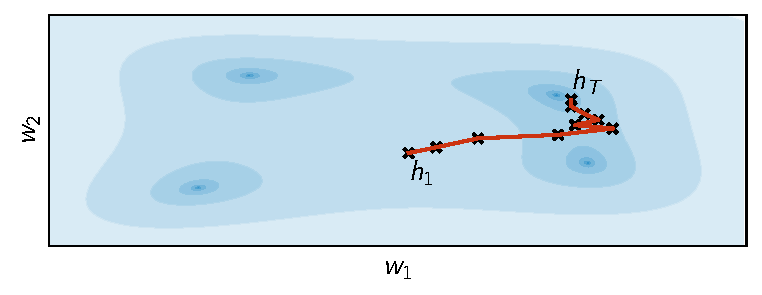
\includegraphics[width=1.0\linewidth]{figures/perspectives_algo.pdf}
  \end{figure}
\end{minipage}
\hfill
\begin{minipage}{0.35\linewidth}
$f$ $\iff$ learning algorithm\\[0.3cm]
$\h_T = f(\h_1) \quad\text{where}\quad \h_1\sim\P$
\end{minipage}
  
  \begin{xblock}{}
      The expression of the ratio becomes {\scriptsize (with a uniform prior and $f$ bijective)}
      \begin{align*}
      \ln\frac{\AQ(\h_T)}{\P(\h_T)} = -\overbrace{\ln\LB\LN\det \frac{\partial f}{\partial \h_1}\RN\RB}^{\mathclap{\text{\bf Captures the learning dynamic}}}
      \end{align*}
  \end{xblock}
\end{xframe}

%%%%%%%%%%%%%%%%%%%%%%%%%%%%%%%%%%%%%%%%%%%%%%%%%%%%%%%%%%%%%%%%%%%%%%%%%%%%%%%
%%%%%%%%%%%%%%%%%%%%%%%%%%%%%%%%%%%%%%%%%%%%%%%%%%%%%%%%%%%%%%%%%%%%%%%%%%%%%%%
%%%%%%%%%%%%%%%%%%%%%%%%%%%%%%%%%%%%%%%%%%%%%%%%%%%%%%%%%%%%%%%%%%%%%%%%%%%%%%%
%%%%%%%%%%%%%%%%%%%%%%%%%%%%%%%%%%%%%%%%%%%%%%%%%%%%%%%%%%%%%%%%%%%%%%%%%%%%%%%

\appendix

\begin{xtitle}

\vspace{1.5cm}

{\huge Thank you for your attention!}

\vspace{1cm}

{\scriptsize\normalfont
{\bf Main contributions:}\\[0.5cm]
\begin{xitemize}
\item[] \printpublication{ViallardGermainHabrardMorvant2021}
\item[] \printpublication{ViallardVidotHabrardMorvant2021}
\item[] \printpublication{ZantedeschiViallardMorvantEmonetHabrardGermainGuedj2021}
\item[] \printpublication{ViallardEmonetHabrardMorvantZantedeschi2022}
\item[] \printpublication{ViallardGermainHabrardMorvant2022}
\end{xitemize}}

\end{xtitle}

\begin{frame}[t,noframenumbering,allowframebreaks]

\frametitle{Contributions of this Thesis}
\begin{refsection}[publications.bib]
\nocite{*}
{\bf International Conference}\\[0.2cm]
\printbibliography[keyword={conference}]
{\bf International Workshop}\\[0.2cm]
\printbibliography[keyword={workshop}]
{\bf National Conference}\\[0.2cm]
\printbibliography[keyword={nat-conference}]
{\bf Research Report}\\[0.2cm]
\printbibliography[keyword={report}]
\end{refsection}
\end{frame}

%%%%%%%%%%%%%%%%%%%%%%%%%%%%%%%%%%%%%%%%%%%%%%%%%%%%%%%%%%%%%%%%%%%%%%%%%%%%%%%

\begin{frame}[t,noframenumbering,allowframebreaks]
  \frametitle{References}
  \printbibliography[title={References}]
 \end{frame}

\end{document}